\documentclass[a4paper,titlepage]{article}
\usepackage[utf8]{inputenc}
\usepackage[T1]{fontenc}
\usepackage[italian]{babel}

\usepackage[hidelinks]{hyperref}
\usepackage{graphicx}
\usepackage{booktabs}
\usepackage{tabularx}
\usepackage{caption}
\captionsetup{font=small} %imposta il font di tutte le didascalie su small

\title{Riassunto\\
		\textbf{Fondamenti di Internet of Things}\\
		{\Large Prof. Sabrina Sicari -- A.A. 2022/23}
}
\author{Federico Garegnani}
\date{\today}

\begin{document}
	\maketitle
	
	\tableofcontents
	\pagebreak
	
	\section{Progettazione di una WSN}

	La progettazione di una WSN è influenzata dai seguenti fattori
	\begin{itemize}
		\item Reliability (o fault tolerance)
		\item Scalabilità
		\item Costi di produzione
		\item Limitiazioni hardware
		\item Topologia
		\item Ambiente applicativo
		\item Mezzo di trasmissione
		\item Consumo di potenza (o lifetime)
	\end{itemize}
	Analizziamo di seguito ogni parametro nel dettaglio
	
\subsection{Reliability}
	La \emph{tolleranza ai guasti} (\emph{fault tolerance}, \emph{reliability} o \emph{affidabilità}) è la capacità della rete di non interrompere il servizio anche in presenza di guasti.
	Un nodo può rompersi per perdita di potenza, danni fisici o interferenze ambientali ma questo non deve pregiudicare l'operatività di tutta la rete di sensori.
	
	L'affidabilità di un nodo sensore $K$ è modellata mediante una distribuzione di Poisson dalla seguente equazione
	\[ R_k(t) = e^{-\lambda_k t} \] 
	Essa fornisce la probabilità che sia verificata una rottura al tempo $t$,
	$\lambda_k$ rappresenta il tasso di rottura (failure rate).
	
	L'affidabilità di un broadcast range con $N$ nodi sensori è ottenuta nel seguente modo
	\[ R(t) = 1 - \prod_{k=1}^{N} [1 - R_k(t)] \]
	A seconda dell'affidabilità richiesta si possono variare i protocolli e gli algoritmi utilizzati.
	
\subsection{Scalabilità}
	Il numero di sensori in una regione può variare considerevolmente, da pochi e diverse migliaia.
	
	La densità dei sensori è il numero di nodi all'interno del \emph{radio range} $R$
	\[ \mu(R) = \frac{N \pi R^2}{A} \]
	dove $N$ è il numero di sensori all'interno della regione di area $A$, mentre $R$ è il range di trasmissione.

\subsection{Costi di produzione}
	Il costo deve essere basso.
	L'obiettivo è di raggiungere un prezzo inferiore a 1~\$/dispositivo, attualmente il costo varia tra \$25 e \$180.
	
\subsection{Topologia}
	Nella gestione della topologia di una sensor network si distinguono tre fasi
	\begin{enumerate}
		\item \textbf{Pre-deployment e deployment phase}\\
			I sensori possono essere gettati da un aeroplano (\emph{random deployment}) oppure possono essere disposti in modo organizzato (\emph{regualar deployment}).
			Nel caso di sensori mobili questi possono muoversi autonomamente e cercare aree di interesse, compensare  guasti nella rete oppure essere mossi da forze esterne come vento e acqua.
			
		\item \textbf{Post-deployment phase}\\
			Variazioni nella topologia possono verificarsi a seguito di cambiamenti di posizione, problemi di raggiungibilità (a causa di jamming\footnote{Il jamming è l'atto di disturbare volutamente le comunicazioni radio (wireless) facendo in modo che ne diminuisca il rapporto segnale/rumore, indice di chiarezza del segnale, tipicamente trasmettendo sulla stessa frequenza e con la stessa modulazione del segnale che si vuole disturbare.},
			rumore, ostacoli, etc.), energia insufficiente, malfunzionamenti.
		
		\item \textbf{Re-deployment di nodi aggiuntivi}\\
	\end{enumerate}

\subsection{Mezzo trasmissivo}
	I dispositivi possono comunicare tramite onde radio, dispositivi ottici (infrarossi) o acustici.
	
\subsection{Consumo potenza}
	La sorgente di potenza (batteria) è molto limitata ed è il principale fattore che determina il tempo di vita del sensore; in molti scenari non è infatti possibile ricaricare le batterie, risulta quindi importante usare l'energia in modo parsimonioso.
	Spesso i dispositivi vengono dotati di due batterie, una batteria principale con il compito di alimentare il dispositivo ed una batteria tampone per l'invio dei dati raccolti prima del completo scaricamento.
	
	Da questo punto di vista assume importanza anche la scelta dei protocolli utilizzati per la trasmissione dei dati, si parla di \emph{Power Aware Communication Protocols} in quanto devono minimizzare la dimensione dei pacchetti e il numero di pacchetti scambiati.
	Alcuni studi hanno analizzato l'assorbimento energetico di ogni componente di un sensore e si è osservato che le fasi di trasmissione e ricezione risultano essere quelle più energivore (Figura \ref{fig:consumoEnergiaDispositivo}).
	
	\begin{figure}[h]
		\centering
		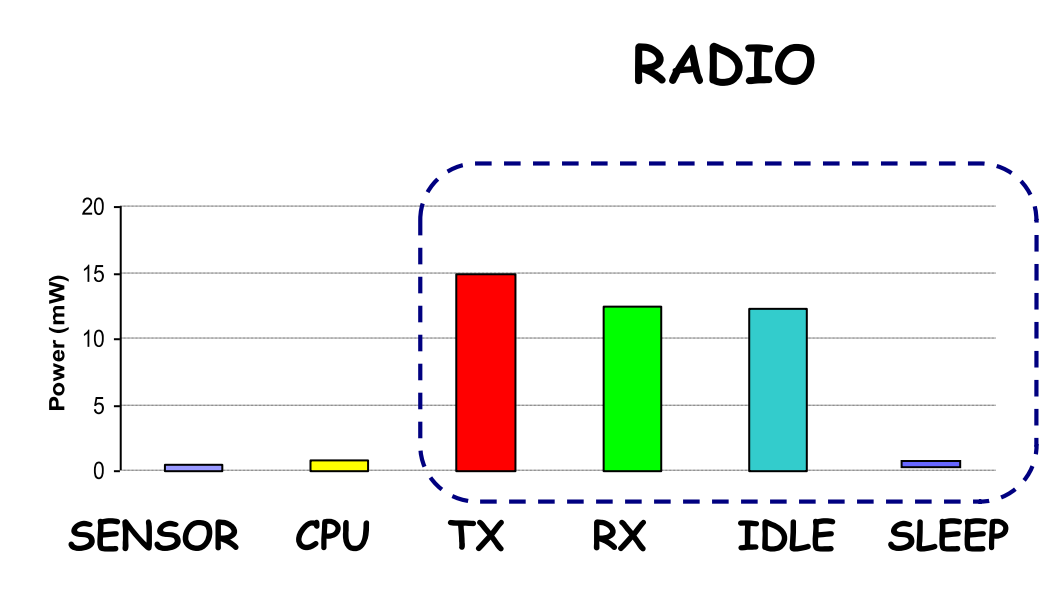
\includegraphics[width=0.7\textwidth]{lez3-progettazione/img/consumoEnergiaDispositivo.png}
		\caption{Consumo di energia per ogni componente del dispositivo}
		\label{fig:consumoEnergiaDispositivo}
	\end{figure}
	
	
	
	
	
	\section{Livello di rete}

	Per una serie di ragioni legate all'elevato numero di nodi, alla limitata potenza e all'approccio data centrico non è possibile utilizzare un identificativo unico per ogni dispositivo all'interno di una sensor network.
	Un indirizzamento dei nodi è tuttavia necessario per la gestione dei nodi, il \emph{querying}, il \emph{service discovery} e il routing.
	
	Risulta necessario utilizzare nuovi algoritmi di routing che tengano conto della limitata potenza, capacità computazionale e memoria disponibili, dei frequenti cambiamenti nella topologia e dell'assenza di un identificativo globale dei dispositivi.
	
\paragraph{Tassonomia dei protocolli di routing}

	Si distinguono tre categorie di protocolli di routing
	\begin{itemize}
		\item Data Centric Protocols\\
			\underline{Flooding}, \underline{Gossiping}, \underline{SPIN}, SAR, \underline{Directed Diffusion}, Rumor Routing, Constrained Anisotropic Diffused Routing, COUGAR, ACQUIRE
		
		\item Hierarchical Protocols\\
			\underline{LEACH}, TEEN, APTEEN, PEGASIS, Energy Aware Scheme
		
		\item Location Based Protocols\\
			MECN, SMECN, GAF, GEAR
	\end{itemize}

\subsection{Flooding e Gossiping}

	Il \emph{flooding} è l'approccio convenzionale e consiste nell'invio broadcast dei dati a tutti i nodi vicini;
	il \emph{gossiping} prevede invece l'invio dei dati a un solo nodo vicino scelto casualmente.
	Sebbene semplici e reattive queste tecniche implicano una serie di svantaggi:
	\begin{itemize}
		\item Implosion
		\item Overlap
		\item Resource Blindness
		\item Power inefficient
	\end{itemize}

	Il gossiping è migliore rispetto al flooding in quanto invia i dati a un solo nodo per risparmiare energia ed evita implosion.
	
\paragraph{Protocollo di routing ideale}
	
	Le caratteristiche che il protocollo idea dovrebbe avere sono:
	\begin{itemize}
		\item selezione del percorso più breve per l'invio dei dati
		\item evitare overlap
		\item minimo consumo di energia
		\item conoscenza globale della topologia
	\end{itemize}

\subsection{SPIN: Sensor Protocol for Information via Negotiation}

	Alla base del protocollo SPIN ci sono due idee: i sensori si scambiano informazioni su dati che sono già in loro possesso o che desiderano avere, risparmiano così energia e lavorano in modo efficiente; i sensori devono monitorare ed adattarsi alle proprie risorse energetiche.
	
	Usa tre tipi di messaggi: ADV, REQ, DATA nel seguente modo:
	\begin{itemize}
		\item quando un sensore ha qualcosa da trasmettere invia in broadcast un \emph{advertisement packet} (ADV)
		\item i nodi interessati invio un \emph{request packet} (REQ)
		\item i dati sono inviati ai nodi che li richiedono
		\item la procedura viene ripetuta finché tutti i nodi non hanno una copia
	\end{itemize}

	SPIN è basato su \emph{data centric routing}, ossia i nodi inviano in broadcast l'advertisement nel caso ci siano dati disponibili e aspettano le richieste delle sink interessate, risulta quindi un ottimo protocollo per disseminare le informazioni tra tutti i nodi.
	
	
	
	
	
	
	
	

	\section{Protocollo SETA}

	Il protocollo SETA (SEcure sharing of TAsks in clustered wireless sensors networks) nasce al fine di garantire sicurezza e privacy all'interno delle rete di sensori, senza sacrificare il risparmio energetico.
	La principale caratteristica che caratterizza e distingue SETA è l'adozione di un'architettura ibrida (wireless sensors network, wireless mesh network), i nodi sensori sono organizzati in cluster e comunicano con i cluster heads, i quali sono i router in grado di comunicare con la sink (Figura \ref{fig:architetturaReteSETA}).
	SETA mira a fornire integrità dei dati, anonimato, risparmio energetico e aggregazione dei dati sicura di tipo end-to-end.
	
	\begin{figure}
		\centering
		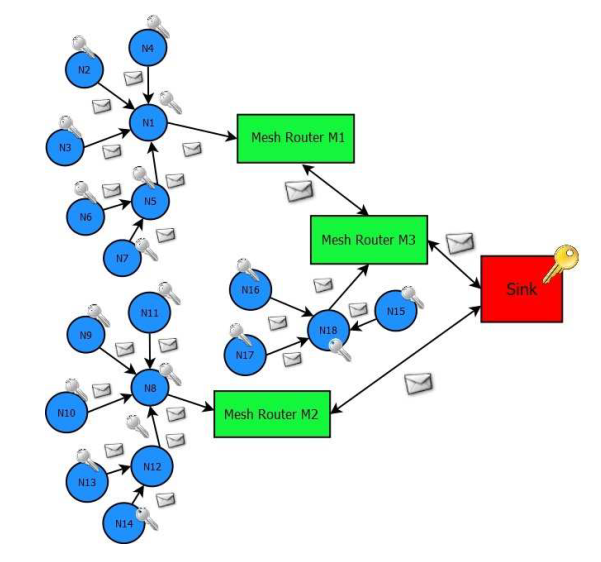
\includegraphics[width=0.5\textwidth]{lez6-SETA/SETA_NetworkModel.png}
		\caption{Architettura di rete del protocollo SETA}
		\label{fig:architetturaReteSETA}
	\end{figure}
	
\paragraph{Aspetti chiave}
	Condivisione dei compiti sulla base delle diverse disponibilità energetiche e capacità computazionali tra sensori e cluster head.
	I nodi sensori svolgono il ruolo di soggetto e processore, si occupano solamente di registrare il dato e criptarlo;
	i cluster head svolgono il ruolo di soggetto nell'aggregare i dati, di processore nella criptazione dei dati e di controller nella verifica dell'integrità dei dati ricevuti.
	
\paragraph{Procedura di trasmissione}
	\begin{enumerate}
		\item I nodi sensori acquisiscono i dati dall'ambiente, li criptano e li inviano al CH
		\item Ogni CH attraversato verifica l'integrità dei dati
		\item La sink decifra i dati e genera le statistiche
	\end{enumerate}

	La verifica di integrità è svolta dal CH nel seguente modo:
	in caso di violazione della privacy viene inviata alla sink una notifica di errore,
	altrimenti il dato può essere aggregato o meno a seconda del livello di congestione della rete e inviato alla sink.\\
	L'assegnamento del ruolo di controllore di sicurezza ai CH riduce il traffico sulla rete e di conseguenza l'overhead, con un sensibile risparmio energetico.
	Gli aspetti negativi della congestione di rete sono lo spreco energetico e la compromissione dell'accuratezza delle stime.
	Ogni qual volta il numero di messaggi del buffer in trasmissione supera una certa soglia, il CH aggrega i dati al fine di evitare l'overflow del buffer; l'aggregazione dei dati è possibile senza che i messaggi vengano decriptati grazie a un algoritmo di \emph{homomorphic enryption}.
	
	 %possibile inserire dettagli sulla struttura del messaggio
	 
\paragraph{Valuzione delle prestazioni}
	In simulazione SETA è stato confrontato con DyDAP: in condizioni ideali DyDAP presenta prestazione migliori, situazione che però si inverte in presenza di nodi malevoli, dove SETA è in grado di generare un minor carico sulla rete;
	SETA è in grado di garantire una maggior accuratezza dei dati in seguito ad aggregazione; 
	DyDAP presenta un leggere vantaggio nei tempi di consegna dei messaggi alla sink;
	SETA garantisce un consumo energetico sensibilmente inferiore.
	
	
	
	
	
	
	
	
	
	
	

	
	\section{Wireless Multimedia Sensors Networks (WMSN)}

	La disponibilità di videocamere e microfoni miniaturizzati ha permesso la nascita delle reti di sensori multimediali, in cui vengono trasmessi segnali audio-video dell'ambiente che si desidera monitorare.
	L'alto volume di flussi multimediali insieme con la ricchezza di informazione generano problemi di congestione, privacy e sicurezza all'interno della rete.
	La prima sfida da affrontare è quella di limitare gli effetti della perdita di pacchetti, un pacchetto perso infatti non solo peggiora la qualità del segnale audio-video ricostruito, ma aumenta anche il consumo energetico a causa della ritrasmissione.
	
	I parametri da monitorare per evitare la congestione della rete sono: carico del canale, tempo di arrivo tra i pacchetti, occupazione del buffer locale.
	
	
\subsection{Secure Selective Dropping Congestion Control (S\textsuperscript{2}DCC)}

	Il protocollo S\textsuperscript{2}DCC mira a risolvere i problemi sopra elencati relativamente alle reti wireless di sensori.
	La prima innovazione è l'azione di tecniche di codifica scalabili, il contenuto multimediale viene infatti trasmesso con differenti flussi  di bit che possono essere sommati tra di loro o ignorati per modificare la risoluzione a seconda della banda disponibile (Figura \ref{fig:WMSN-trasmissioneBitstreams}).
	Il protocollo è poi in grado di garantire sicurezza e supporta sia WMSN gerarchiche che ibride, permettendo la distribuzione dei compiti nella rete sulla base delle capacità di ogni nodo.
	
	\begin{figure}
		\centering
		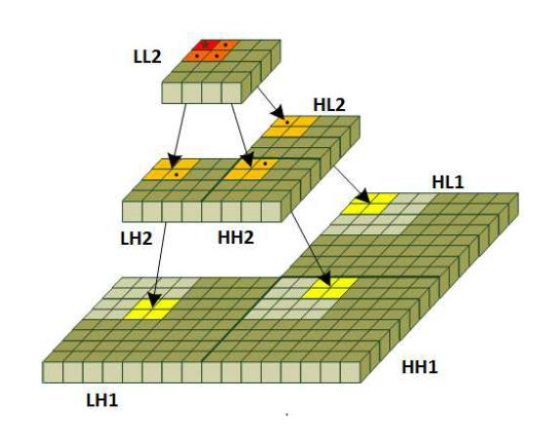
\includegraphics[width=0.5\textwidth]{lez7/differentBitstreamsVideoVMSN.png}
		\caption{Trasmissione video su una WMSN con differenti bitstreams (codec FS-SPIHT)}
		\label{fig:WMSN-trasmissioneBitstreams}
	\end{figure}

	\section{Radio Frequency Identification (RFID)}

	L'idea di RFID si è sviluppata come evoluzione elettronica dei codici a barre, per un'identificazione più rapida dei beni.
	
	La rete RFID si basa sulla presenza di due dispositivi di base: un lettore e un tag.
	Un lettore è composto da modulo a radiofrequenza (antenna), memoria, CPU, Batteria;
	un tag è composto da antenna, circuito di recupero dell'energia (trasmessa dal lettore), memoria non volatile per memorizzare l'ID, e in alcuni casi anche di sensori e una piccola CPU.
	Si distinguono 3 tipi di tag:
	\begin{description}
		\item[Passivi] Funzionano solo grazie al circuito di recupero dell'energia che cattura quella trasmessa dal lettore
		\item[Semi-passivi]  Dotati di batteria
		\item[Attivi] Dotati di batteria e trasmettitore
	\end{description}

	\paragraph{Electronic Product Code (EPC)}
	Ogni tag è dotato di un EPC, si tratta di uno standard che definisce un codice univoco del prodotto su 96 bit organizzati nel seguente modo:
	\begin{itemize}
		\item \textit{Header}. 8 bit, numero di versione del tag
		\item \textit{EPC Manager}. 28 bit, ID del produttore
		\item \textit{Object class}. 24 bit, ID del prodotto
		\item \textit{Serial number}. ID dell'unità
	\end{itemize}

	Le sfide nella realizzazione di un tag RFID sono la costruzione di un circuito di recupero dell'energia efficiente, la miniaturizzazione e il contenimento del costo.
	
	Le sfide nella realizzazione di un lettore RFID riguardano invece la realizzazione di antenne in grado di fornire sufficiente energia al tag, grande differenza nella magnitudo del segnale inviato e ricevuto e l'integrazione con i sistemi industriali più diffusi.
	
	\begin{figure}[h]
		\centering
		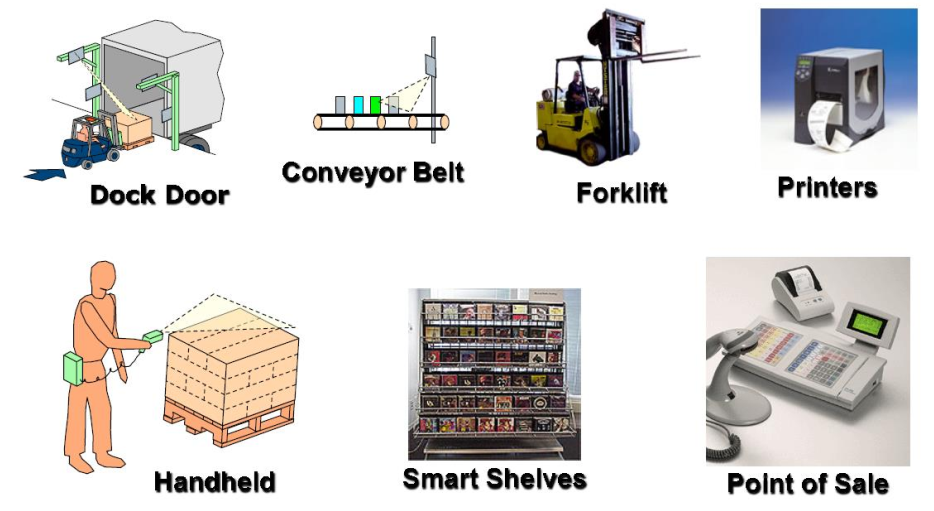
\includegraphics[width=0.8\textwidth]{lez7/useCasesRFID.png}
		\caption{Applicazioni reali che sfruttano RFID}
		\label{fig:useCasesRFID}
	\end{figure}

	RFID sfrutta le frequenze tra 100 MHz e 1 GHz in quanto risultano essere quelle ottimali per la propagazione del segnale in ambienti affollati (Figura \ref{fig:frequenzaOttimale}).
	
	\begin{figure}[h]
		\centering
		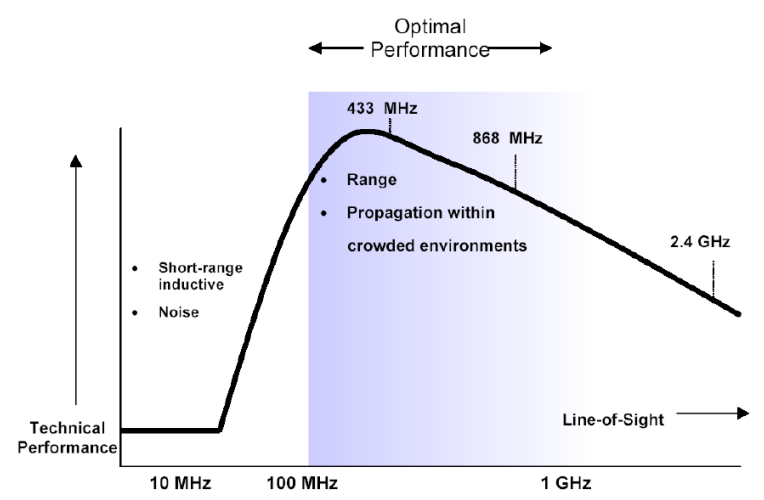
\includegraphics[width=0.6\textwidth]{lez7/optimalFrequency.png}
		\caption{Performance di trasmissione al variare della frequenza per RFID}
		\label{fig:frequenzaOttimale}
	\end{figure}


\section{Near Field Communication (NFC)}

	\paragraph{Connessione tra due dispositivi}
	\begin{enumerate}
		\item La bobina nel primo dispositivo è attraversata da una corrente che genera un campo magnetico percepito dal secondo dispositivo
		\item il secondo dispositivo identifica il campo magnetico ricevuto come un segnale valido e offre la connessione
		\item il primo dispositivo accetta la connessione e inizia la transazione
	\end{enumerate}

	Grazie ai dispositivi dotati di NFC gli utenti possono
	eseguire pagamenti o usare coupon tramite il dispositivo, senza estrarre la carta di credito o debito;
	trasferire file;
	scaricare informazioni circa oggetti, servizi o luoghi;
	mostrare documenti digitale come le carte di imbarco.
	
	I rischi legati all'utilizzo di questa tecnologia sono essenzialmente legati
	alla privacy (quali dati vengono trasmessi, processati e memorizzati?),
	alla sicurezza (cosa succede se smarrisco lo smarthphone?)
	e al \emph{sentinel hacking}, in cui un tag NFC potrebbe essere nascosto in un punto e registrare le informazioni degli smartphone con cui viene in contatto.
	
	I principali vantaggi della tecnologia NFC restano comunque la comunicazione bi-direzionale, l'alto livello di sicurezza grazie alle tecniche di cifratura, l'alta velocità di riconoscimento con una minima probabilità di errore.
	
	\paragraph{Alternative}
	Un'alternativa a NFC sono i codici a barre o i codici QR.
	Ognuna di queste tecnologie presenta comunque alcuni punti di forza, motivo per cui NFC non mira a sostituire i lettori ottici.
	In Figura \ref{fig:comparazioneRFID-barcode} è riportato un confronto.
	
	\begin{figure}[h]
		\centering
		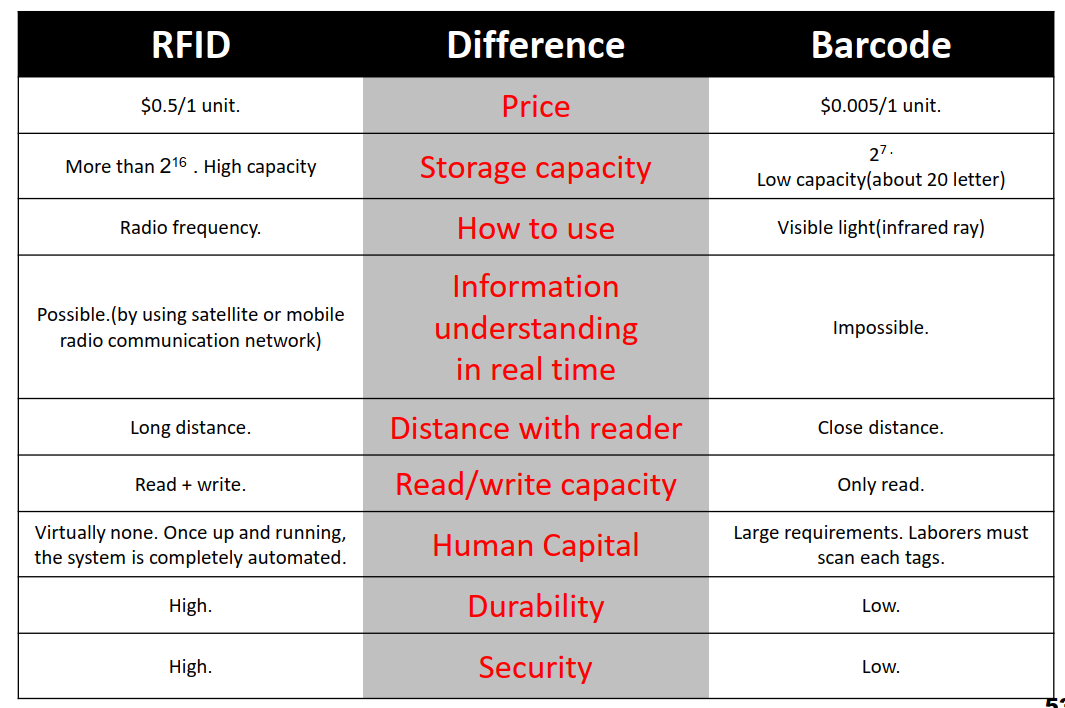
\includegraphics[width=0.8\textwidth]{lez7/tabellaComparativaRFID-barcode.png}
		\caption{Comparazione tra RFID e codici a barre}
		\label{fig:comparazioneRFID-barcode}
	\end{figure}

	\section{Nanotecnologie}

	La nanotecnologia è un ramo della scienza applicata e della tecnologia che si occupa del controllo della materia su scala dimensionale nell'ordine del nanometro e della progettazione e realizzazione di dispositivi in tale scala.
	
	La nascita di questa nuova branca della tecnologia ci pone subito di fronte ad alcuni rischi, quali effetti avversi sulla salute umana o sull'ambiente in seguito ad un'esposizione volontaria o accidentale e la potenziale proprietà esplosiva delle nanostrutture.
	Risulta molto difficile fare una valutazione dei rischi associati a questa tecnologia per diversi fattori,
	in primo luogo c'è bisogno di personale specializzato e apparecchiature sofisticate;
	risulta poi difficile prevedere come determinate particelle si comporteranno una volta ingerite o disperse nell'ambiente; infine bisogna valutare la potenziale presenza di sostanze tossiche e la loro persistenza all'interno del corso o in natura.
	
	Al momento sono attive due grosse aree di ricerca: \emph{Electromagnetic Nano Communication} e \emph{comunicazione molecolare}.
	Nella comunicazione molecolare (\emph{molecular communication}) l'informazione è codificata all'interno di DNA, proteine, peptidi, etc ed è trasmessa per diffusione o trasporto attivo\footnote{Il trasporto attivo è il trasporto di molecole attraverso la membrana plasmatica mediato da una proteina transmembrana detta trasportatore di membrana.
		A differenza di quanto avviene nel trasporto passivo, nel trasporto attivo è richiesta una spesa energetica ed è sempre necessaria la mediazione di un trasportatore.
		In questa forma di trasporto le molecole si muovono contro un gradiente elettrico, chimico o elettrochimico.}.
	
	Nella comunicazione elettromagnetica si viene invece a creare una BAN (Body Area Network), composta da molti sensori che comunicano con un micro-gateway (tramite frequenze nell'ordine del THz).
\end{document}